\documentclass[a4paper,11pt,fleqn,dvipsnames,oneside,openright,oldfontcommands]{memoir} 	% Openright aabner kapitler paa hoejresider (openany begge)


%%%%%%%%% Indsat random
%makes it possible to refer to the name of a chapter rather than just the number.
\usepackage{nameref}
\usepackage{pdfpages}
\usepackage{marvosym}
\usepackage{setspace}
\usepackage{graphicx} % For at sætte 2 billeder ved siden af hinanden

%package for writing program code in latex
\usepackage{listings}
%%%%%%%%%%%%%%%%%%%%%%

% ¤¤ Oversaettelse og tegnsaetning ¤¤ %
\usepackage[T1]{fontenc}					% Output-indkodning af tegnsaet (T1)
\usepackage[danish]{babel}					% Dokumentets sprog
\usepackage[utf8]{inputenc}					% Input-indkodning af tegnsaet (UTF8)
\usepackage{ragged2e,anyfontsize}			% Justering af elementer
\usepackage{fixltx2e}						% Retter forskellige fejl i LaTeX-kernen							
				
																							
% ¤¤ Figurer og tabeller (floats) ¤¤ %
\usepackage{graphicx} 						% Haandtering af eksterne billeder (JPG, PNG, EPS, PDF)
%\usepackage{eso-pic}						% Tilfoej billedekommandoer paa hver side
%\usepackage{wrapfig}						% Indsaettelse af figurer omsvoebt af tekst. \begin{wrapfigure}{Placering}{Stoerrelse}
\usepackage{multirow}                		% Fletning af raekker og kolonner (\multicolumn og \multirow)
\usepackage{multicol}         	        	% Muliggoer output i spalter
\usepackage{rotating}						% Rotation af tekst med \begin{sideways}...\end{sideways}
\usepackage{colortbl} 						% Farver i tabeller (fx \columncolor og \rowcolor)
\usepackage{xcolor}							% Definer farver med \definecolor. Se mere: http://en.wikibooks.org/wiki/LaTeX/Colors
\usepackage{flafter}						% Soerger for at floats ikke optraeder i teksten foer deres reference
\let\newfloat\relax 						% Justering mellem float-pakken og memoir
\usepackage{float}							% Muliggoer eksakt placering af floats, f.eks. \begin{figure}[H]
\usepackage{array,booktabs,xcolor,longtable} % kan lave \hdashline i tabellertabe
\usepackage{arydshln}
\usepackage{tabu}

	
	
% ¤¤ Matematik mm. ¤¤
\usepackage{amsmath , amsthm , amsfonts , amssymb, float, stmaryrd} 		% Avancerede matematik-udvidelser
%\usepackage{mathtools}						% Andre matematik- og tegnudvidelser
\usepackage{textcomp}                 		% Symbol-udvidelser (f.eks. promille-tegn med \textperthousand )
\usepackage{rsphrase}						% Kemi-pakke til RS-saetninger, f.eks. \rsphrase{R1}
\usepackage[version=3]{mhchem} 				% Kemi-pakke til flot og let notation af formler, f.eks. \ce{Fe2O3}
\usepackage{siunitx}						% Flot og konsistent praesentation af tal og enheder med \si{enhed} og \SI{tal}{enhed}
\sisetup{output-decimal-marker = {,}}		% Opsaetning af \SI (DE for komma som decimalseparator) 

% ¤¤ Referencer og kilder ¤¤ %
\usepackage[danish]{varioref}				% Muliggoer bl.a. krydshenvisninger med sidetal (\vref)
\usepackage[numbers]{natbib}				% Udvidelse med naturvidenskabelige citationsmodeller
%\usepackage{xr}							% Referencer til eksternt dokument med \externaldocument{<NAVN>}
%\usepackage{glossaries}					% Terminologi- eller symbolliste (se mere i Daleifs Latex-bog)
\usepackage{lastpage}					% Gør det mulig at refere til sidste side 

% ¤¤ Misc. ¤¤ %
\usepackage{listings}						% Placer kildekode i dokumentet med \begin{lstlisting}...\end{lstlisting}
\usepackage{lipsum}							% Dummy text \lipsum[..]
\usepackage[shortlabels]{enumitem}			% Muliggoer enkelt konfiguration af lister
\usepackage{pdfpages}						% Goer det muligt at inkludere pdf-dokumenter med kommandoen \includepdf[pages={x-y}]{fil.pdf}	
\pdfoptionpdfminorversion=6					% Muliggoer inkludering af pdf dokumenter, af version 1.6 og hoejere
\pretolerance=2500 							% Justering af afstand mellem ord (hoejt tal, mindre orddeling og mere luft mellem ord)


% Kommentarer og rettelser med \fxnote. Med 'final' i stedet for 'draft' udloeser hver note en error i den faerdige rapport.
\usepackage[footnote,draft,danish,silent,nomargin]{fixme}		


%%%% CUSTOM SETTINGS %%%%

% ¤¤ Marginer ¤¤ %
\setlrmarginsandblock{3.0cm}{2.5cm}{*}		% \setlrmarginsandblock{Indbinding}{Kant}{Ratio}
\setulmarginsandblock{2.5cm}{3.0cm}{*}		% \setulmarginsandblock{Top}{Bund}{Ratio}
\checkandfixthelayout 						% Oversaetter vaerdier til brug for andre pakker

%	¤¤ Afsnitsformatering ¤¤ %
\setlength{\parindent}{6mm}           		% Stoerrelse af indryk
\setlength{\parskip}{0mm}          			% Afstand mellem afsnit ved brug af double Enter
\linespread{1,1}							% Linie afstand



% ¤¤ Indholdsfortegnelse ¤¤ %
\setsecnumdepth{subsection}		 			% Dybden af nummerede overkrifter (part/chapter/section/subsection)
\maxsecnumdepth{subsection}					% Dokumentklassens graense for nummereringsdybde
\settocdepth{subsection} 					% Dybden af indholdsfortegnelsen

% ¤¤ Lister ¤¤ %
\setlist{
  topsep=0pt,								% Vertikal afstand mellem tekst og listen
  itemsep=-1ex,								% Vertikal afstand mellem items
} 

%hyperlinks in the tabel of contents - comment this out before the report is printed.
\usepackage{hyperref}
\hypersetup{
	bookmarks = true,  % Show 'bookmark'-frame in pdf.
	colorlinks = true, % True = colored links, False = framed links.
	citecolor = black,  % Link color for references.
	linkcolor = black,  % Link color in table of contents.
	urlcolor = black,   % Link color for extern URLs.
}

% ¤¤ Opsaetning af figur- og tabeltekst ¤¤ %
\usepackage{caption}
%\usepackage{subcaption}
\captionnamefont{\small\bfseries\itshape}	% Opsaetning af tekstdelen ('Figur' eller 'Tabel')
\captiontitlefont{\small}					% Opsaetning af nummerering
\captiondelim{. }							% Seperator mellem nummerering og figurtekst
\hangcaption								% Venstrejusterer flere-liniers figurtekst under hinanden
%\captionwidth{0.9\textwidth}					% Bredden af figurteksten
\setlength{\belowcaptionskip}{0pt}			% Afstand under figurteksten
\captionsetup[figure]{labelfont={bf,it},font={it}} % sætter nummer til fed og kursis. Resten til fed + skriften er mindre end resten
\captionsetup[table]{labelfont={bf,it},font={it}} 


% ¤¤ Opsaetning af listings ¤¤ %

\definecolor{commentGreen}{RGB}{34,139,24}
\definecolor{stringPurple}{RGB}{208,76,239}

\lstset{language=Matlab,					% Sprog
	basicstyle=\ttfamily\scriptsize,		% Opsaetning af teksten
	keywords={for,if,while,else,elseif,		% Noegleord at fremhaeve
			  end,break,return,case,
			  switch,function},
	keywordstyle=\color{blue},				% Opsaetning af noegleord
	commentstyle=\color{commentGreen},		% Opsaetning af kommentarer
	stringstyle=\color{stringPurple},		% Opsaetning af strenge
	showstringspaces=false,					% Mellemrum i strenge enten vist eller blanke
	numbers=left, numberstyle=\tiny,		% Linjenumre
	extendedchars=true, 					% Tillader specielle karakterer
	columns=flexible,						% Kolonnejustering
	breaklines, breakatwhitespace=true,		% Bryd lange linjer
}

% ¤¤ Navngivning ¤¤ %
\addto\captionsdanish{
	\renewcommand\appendixname{Bilag}
	\renewcommand\contentsname{Indholdsfortegnelse}	
	\renewcommand\appendixpagename{Bilag}
	\renewcommand\appendixtocname{Bilag}
	\renewcommand\cftchaptername{\chaptername~}				% Skriver "Kapitel" foran kapitlerne i indholdsfortegnelsen
	\renewcommand\cftappendixname{\appendixname~}			% Skriver "Appendiks" foran appendiks i indholdsfortegnelsen
}

% ¤¤ Kapiteludssende ¤¤ %
%\definecolor{numbercolor}{gray}{0.7}		% Definerer en farve til brug til kapiteludseende
%\newif\ifchapternonum

\makechapterstyle{AAU}
{
	% Afstand mellem sidehovedet og kapitel+tal+kapitelnavnet defineres til:
	\setlength{\beforechapskip}{0cm}

	% Afstanden mellem kapitelnavnet og body-teksten defineres til:
	\setlength{\afterchapskip}{2cm}

	% Typografiopsætningen til kapitel+tal defineres til:
	\renewcommand\chapnamefont{\sffamily\bfseries\LARGE\raggedright}
	
	% Typografiopsætningen til kapitel+tal defineres til:
	\renewcommand\chaptitlefont{\sffamily\bfseries\huge\color[cmyk]{1.00,0.38,0.00,0.64}}

	% Forårsager, at der til kapitlet også tilføjes dets respektive tal:
	\renewcommand\chapternamenum{}
	\renewcommand\printchapternum
	{
		\makebox[0pt][l]
		{
			\color[cmyk]{1.00,0.38,0.00,0.64}
			\hspace{0.1cm}
			\resizebox{!}{1cm}{\chapnamefont\bfseries\sffamily\thechapter}
		}
	}
	
	% Definitionen af linjenstykket mellem ``Kapitel #'' samt ``kapitelnavnet'':
			\renewcommand\afterchaptertitle{\par\hspace{1.5cm}\hrule height 1pt\vskip\midchapskip}
}

% Aktivering af selve kapitellayoutet med dét navn, som definerer kapitellayoutet (ses fra tidligere):
\chapterstyle{AAU}

%\makechapterstyle{jenor}{					% Definerer kapiteludseende frem til ...
%  \renewcommand\beforechapskip{0pt}
%  \renewcommand\printchaptername{}
%  \renewcommand\printchapternum{}
% % \renewcommand\printchapternonum{\chapternonumtrue}
%  \renewcommand\chaptitlefont{\fontfamily{pbk}\fontseries{db}\fontshape{n}\fontsize{20}{25}\selectfont\raggedright}
%  \renewcommand\chapnumfont{\fontfamily{pbk}\fontseries{m}\fontshape{n}\fontsize{1in}{0in}\selectfont\color{numbercolor}}
% \renewcommand\printchaptertitle[1]{
%    \noindent
%    \ifchapternum
%     \begin{tabularx}{\textwidth}{XI}
%	{\let\\\newline\chaptitlefont ##1\par}     
%    \end{tabularx}
%    \par\vskip-2.5mm\hrule
%    \else
%    \begin{tabularx}{\textwidth}{X}
%      {\parbox[b]{\linewidth}{\chaptitlefont ##1}} & \raisebox{-15pt}{\chapnumfont \thechapter}
%    \end{tabularx}
%    \par\vskip2mm\hrule
%    \fi
%  }
%}											% ... her
%
%\chapterstyle{jenor}						% Valg af kapiteludseende - Google 'memoir chapter styles' for alternativer

% ¤¤ Sidehoved ¤¤ %

\makepagestyle{AAU}							% Definerer sidehoved og sidefod udseende frem til ...
\makepsmarks{AAU}{%
	\createmark{chapter}{left}{shownumber}{}{. \ }
	\createmark{section}{right}{shownumber}{}{. \ }
	\createplainmark{toc}{both}{\contentsname}
	\createplainmark{lof}{both}{\listfigurename}
	\createplainmark{lot}{both}{\listtablename}
	\createplainmark{bib}{both}{\bibname}
	\createplainmark{index}{both}{\indexname}
	\createplainmark{glossary}{both}{\glossaryname}
}
\nouppercaseheads											% Ingen Caps oenskes

\makeoddhead{AAU}{Gruppe 16gr5404}{}{\leftmark}				% Definerer lige siders sidehoved (\makeevenhead{Navn}{Venstre}{Center}{Hoejre})
\makeevenhead{AAU}{\rightmark}{}{Aalborg Universitet}		% Definerer ulige siders sidehoved (\makeoddhead{Navn}{Venstre}{Center}{Hoejre})
\makeevenfoot{AAU}{Side \thepage\ af \pageref{LastPage}}{}{}							% Definerer lige siders sidefod (\makeevenfoot{Navn}{Venstre}{Center}{Hoejre})
\makeoddfoot{AAU}{}{}{Side \thepage\ af \pageref{LastPage}}								% Definerer ulige siders sidefod (\makeoddfoot{Navn}{Venstre}{Center}{Hoejre})
\makeheadrule{AAU}{\textwidth}{0.5pt}						% Tilfoejer en streg under sidehovedets indhold
\makefootrule{AAU}{\textwidth}{0.5pt}{1mm}					% Tilfoejer en streg under sidefodens indhold

\copypagestyle{AAUchap}{AAU}								% Sidehoved for kapitelsider defineres som standardsider, men med blank sidehoved
\makeoddhead{AAUchap}{}{}{}
\makeevenhead{AAUchap}{}{}{}
\makeheadrule{AAUchap}{\textwidth}{0pt}
\aliaspagestyle{chapter}{AAUchap}							% Den ny style vaelges til at gaelde for chapters
															% ... her
															
\pagestyle{AAU}												% Valg af sidehoved og sidefod


%%%% CUSTOM COMMANDS %%%%

% ¤¤ Billede hack ¤¤ %
\newcommand{\figur}[4]{
		\begin{figure}[H] \centering
			\includegraphics[width=#1\textwidth]{billeder/#2}
			\caption{#3}\label{#4}
		\end{figure} 
}

% ¤¤ Specielle tegn ¤¤ %
\newcommand{\decC}{^{\circ}\text{C}}
\newcommand{\dec}{^{\circ}}
\newcommand{\m}{\cdot}


%%%% ORDDELING %%%%

\hyphenation{}

%%%%Fra engelsk til dansk i \autoref{•} %%%%
\renewcommand{\figureautorefname}{figur}
\renewcommand{\sectionautorefname}{afsnit}
\renewcommand{\subsectionautorefname}{afsnit}
\renewcommand{\subsubsectionautorefname}{afsnit}
\renewcommand{\tableautorefname}{tabel}
\renewcommand{\appendixautorefname}{bilag}
\renewcommand{\equationautorefname}{ligning}
\renewcommand{\itemautorefname}{punkt}
\renewcommand{\chapterautorefname}{kapitel}
%Figure references:
\newcommand{\figref}[1]{figur \ref{#1}}

%Figure references after full stop/period:
\newcommand{\Figref}[1]{Figur \ref{#1}}

%Table references:
\newcommand{\tabref}[1]{tabel \ref{#1}}

%Table references after full stop/period:
\newcommand{\Tabref}[1]{Tabel \ref{#1}}

%Section references:
\newcommand{\secref}[1]{afsnit \ref{#1} på side \pageref{#1}}

%Section references:
\newcommand{\Secref}[1]{Afsnit \ref{#1} på side \pageref{#1}}

%Appendix references:
\newcommand{\appref}[1]{appendiks \ref{#1} på side \pageref{#1}}

%Appendix references:
\newcommand{\Appref}[1]{Appendiks \ref{#1} på side \pageref{#1}}

%chapter references: 
\newcommand{\chapref}[1]{kapitel \ref{#1} på side \pageref{#1}}

%chapter references: 
\newcommand{\Chapref}[1]{Kapitel \ref{#1} på side \pageref{#1}}

%Units:
%\newcommand{\unit}[1]{&& \left[\si{#1}\right]}

%Text:
\newcommand{\tx}[1]{\text{#1}}

%Equation references:
%1 equation:
\renewcommand{\eqref}[1]{ligning (\ref{#1})}
%2 equations:
%\newcommand{\eqrefTwo}[2]{ligning (\ref{#1})} and \textbf{(\ref{#2})}
%%3 equations:
%\newcommand{\eqrefThree}[3]{ligning (\ref{#1})}, \textbf{(\ref{#2})} and \textbf{(\ref{#3})}
%%4 equations:
%\newcommand{\eqrefFour}[4]{ligning (\ref{#1})}, \textbf{(\ref{#2})}, \textbf{(\ref{#3})} and \textbf{(\ref{#4})}
%%5 equations:
%\newcommand{\eqrefFive}[5]{ligning (\ref{#1})}, \textbf{(\ref{#2})}, \textbf{(\ref{#3})}, \textbf{(\ref{#4})} and \textbf{(\ref{#5})}
%%5 equations:
%\newcommand{\eqrefSix}[6]{ligning (\ref{#1})}, \textbf{(\ref{#2})}, \textbf{(\ref{#3})}, \textbf{(\ref{#4})}, \textbf{(\ref{#5})} and \textbf{(\ref{#6})}
%%5 equations:
%\newcommand{\eqrefSeven}[7]{ligning (\ref{#1})}, \textbf{(\ref{#2})}, \textbf{(\ref{#3})}, \textbf{(\ref{#4})}, \textbf{(\ref{#5})}, \textbf{(\ref{#6})} and \textbf{(\ref{#7})}
%
%%Equation references after full stop/period:
%%1 equation:
%\newcommand{\Eqref}[1]{Ligning (\ref{#1})}
%%2 equations:
%\newcommand{\EqrefTwo}[2]{Ligning (\ref{#1})} and \textbf{(\ref{#2})}
%%3 equations:
%\newcommand{\EqrefThree}[3]{Ligning (\ref{#1})}, \textbf{(\ref{#2})} and \textbf{(\ref{#3})}
%%4 equations:
%\newcommand{\EqrefFour}[4]{Ligning (\ref{#1})}, \textbf{(\ref{#2})}, \textbf{(\ref{#3})} and \textbf{(\ref{#4})}
%%5 equations:
%\newcommand{\EqrefFive}[5]{Ligning (\ref{#1})}, \textbf{(\ref{#2})}, \textbf{(\ref{#3})}, \textbf{(\ref{#4})} and \textbf{(\ref{#5})}
%%5 equations:
%\newcommand{\EqrefSix}[6]{Ligning (\ref{#1})}, \textbf{(\ref{#2})}, \textbf{(\ref{#3})}, \textbf{(\ref{#4})}, \textbf{(\ref{#5})} and \textbf{(\ref{#6})}
%%5 equations:
%\newcommand{\EqrefSeven}[7]{Ligning (\ref{#1})}, \textbf{(\ref{#2})}, \textbf{(\ref{#3})}, \textbf{(\ref{#4})}, \textbf{(\ref{#5})}, \textbf{(\ref{#6})} and \textbf{(\ref{#7})}
\raggedbottom % Soerger for at LaTeX ikke "straekker" teksten

\begin{document}

%-------------Formaliteter-------------------
\frontmatter	 
\clearpage
\thispagestyle{empty}

\begin{figure}[H]
	\raggedleft
		
\includegraphics[width=0.2\textwidth]{figures/aaulogo-da.png}
\end{figure} 
\vspace*{\fill} 
\begin{center}
\begin{Huge}
\textbf{Registrering og objektivisering af fysisk aktivitetsniveau hos kronikere i almen praksis via aktivitetsarmbånd}\\
\vspace{5 mm}
5. semesterprojekt - Efterår $2016$\\
\vspace{3 mm}
\end{Huge}
{\Large Gruppe $16$gr$5404$}
\begin{figure}[H]
	\centering
	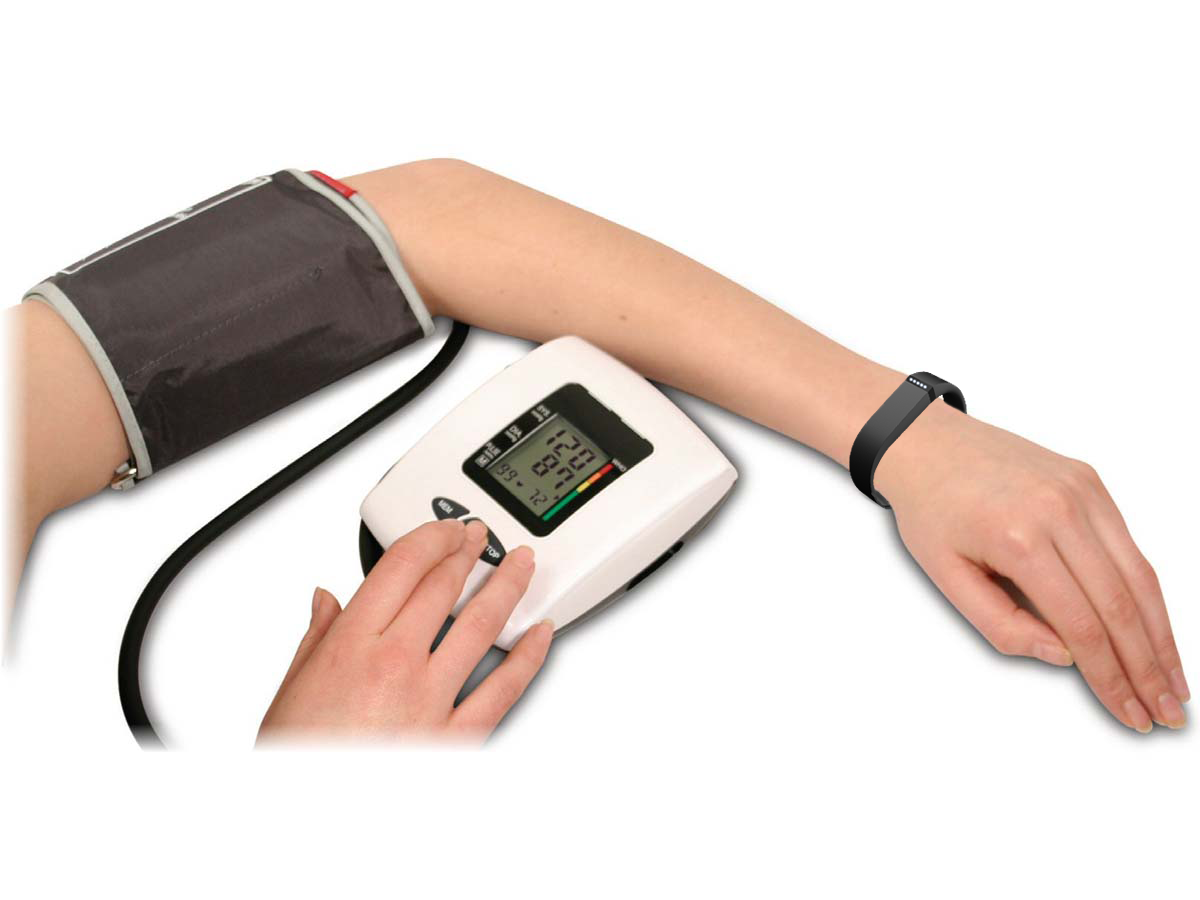
\includegraphics[width=0.8\textwidth]{figures/forside}
\end{figure}	
\end{center}
\vspace*{\fill}

\begin{center}
\line(1,0){400}
\end{center}
%\begin{document} 
\thispagestyle{empty}
%\begin{titlepage}
\begin{nopagebreak}
{\samepage 

\begin{tabular}{r}
\parbox{\textwidth}{ 
 {
\includegraphics[height=2.5cm]{figures/aaulogo-da.png}}
\hfill \hspace{2cm} \parbox{8cm}
{\begin{tabular}{l} %4.90
{\small \textbf{5. semester}}\\
{\small \textbf{School of Medicine and Health}}\\
%{\small \textbf{\textcolor{MidnightBlue}{}}}\\ 
{\small \textbf{Sundhedsteknologi}}\\
{\small Fredrik Bajers Vej $7$A} \\
{\small $9220$ Aalborg} \\
%{\small \textcolor{NavyBlue}{\emph{http://www.smh.aau.dk/}}}
\end{tabular}}}
\end{tabular}

\hspace{-1.5cm}\begin{tabular}{cc}
\parbox{7cm}{
\begin{description}

\item {Titel:}

Registrering og objektivisering af fysisk aktivitetsniveau hos kronikere i almen praksis via aktivitetsarmbånd\\

\item {Tema:} 


Klinisk teknologi\\

\end{description}

\parbox{8cm}{

\begin{description}
\item {Projektperiode:}\\
   Efteråret $2016$\\
   $02/09/2016$ - $19/12/2016$\\
   
\item {Projektgruppe:}\\
  $16$gr$5404$\\
  
\item {Medvirkende:}\\
Birgithe Kleemann Rasmussen\\
Mads Kristensen\\
Signe Hejgaard Kristoffersen\\
Simon Bruun\\
Suado Ali Haji Diriyi\\
Toby Steven Waterstone

\hspace{2cm}
\item {Vejledere:}\\
Ole Hejlesen, Morten Sig Ager Jensen \\
og Mads Nibe Stausholm\\
\end{description}

}\\
\begin{description}
\item {Sider: ??} \\
%\item {Appendikser: ??}\\
\hspace{1.5cm}
%\item {Afsluttet: $27/05/2016$}
\end{description}
\vfill } &
\parbox{7cm}{
  \vspace{.15cm}
  \hfill 
  \begin{tabular}{l}
  {Synopsis:}\bigskip \\
  \fbox{
    \parbox{9cm}{\bigskip
     {\vfill{\small Denne rapport belyser idéen af at anvende et aktivitetsarmbånd til monitorering af hypertensive patienters aktivitetsniveau. 
Hypertension er en folkesygdom, og i Danmark er det vurderet, at 20 \% har sygdommen. Disse patienter anbefales fysisk aktivitet som en del af behandlingen, da dette resulterer i et reduceret blodtryk, hvorpå risikoen for følgesygdomme og medicinering ligeledes kan reduceres eller udskydes. 
Formålet har således været at undersøge et udvalgt aktivitetsarmbånd, Fitbit Flex, og vurdere, om dette hensigtsmæssigt kan anvendes i behandlings- og/eller udredningsforløb af hypertension. 
Den registrerede aktivitet vil give læger og andet relevant sundhedsfagligt personale indblik i patienters aktivitetsniveau, hvorved en korrekt rådgivning kan gives til patienten. 

Vurderingen af Fitbit Flex som registrering- og objektiviseringsmetode er fortaget med udgangspunkt i metoden for en medicinsk teknologi vurdering.  

På baggrund af flere studier er det vist at aktivitetsarmbånd har potentialet til at motivere personer til at være mere fysisk aktive, hvilket vil kunne medføre en gavnlig effekt på hypertensive patienters tilstand. Yderligere ved at data gemmes ved brug af en applikation tilhørende aktivitetsarmbåndet, muliggøres en objektiv monitorering af bæren af armbåndet, hvilket vil kunne give grundlag og viden for lægen, om vejledning og anbefalinger om hvordan patientens behandlingsforløb kan struktureres ved fremtidig behandling.

Implementeringen af aktivitetsarmbånd vil indledningsvist kræve resourser i den primære sundhedssektor, men såfremt aktivitetsarmbånd viser sig effektivt for behandlingen af hypertensive patienter, vil resultatet kunne afspejle sig i et overordnet lettere behandlingsforløb.
     \bigskip}}
     }}
   \end{tabular}}
\end{tabular}} \hspace{-1.5cm}%\vspace{1.0cm}

\vfill
{\footnotesize\itshape \noindent Offentliggørelse af rapportens indhold, med kildeangivelse, må kun ske efter aftale med forfatterne.}
\\
\end{nopagebreak}
%\end{titlepage}
%\end{document}
\chapter{Forord}
Skriv forord her.... 


\section*{Læsevejledning}
Denne rapport består af et initierende problem, en problemanalyse, en problemformulering, MTV-spørgsmål og -analyser samt en syntese af disse analyser, der gerne skal besvare problemformuleringen. 

Det initiernede problem og problemanalysen belyser og analyserer projektets problemstillinger og leder frem til en problemformulering igennem en problemafgrænsning. MTV-spørgsmålene og -analyserne beskæftiger sig med de fire MTV-elementer; patient, teknologi, organisation og økonomi. Syntesen dækker over en diskussion af MTV-analyserne, en konklusion på problemformuleringen samt en perspektivering til valgte teknologi i projektet. 


\subsection*{Kildeangivelse}
I denne rapport bliver kilder angivet ved Vancouver-metoden, hvor kilden henvises til som et nummer i kantede parenteser. Information omkring kilden findes i litteraturlisten.


%Teknologiafsnittet vil beskrive den valgte teknologi, og hvilke variationer af teknologien der eksistere i dag. En sammenligning af variationerne vil blive fortaget, med henblik på at fremhæve fordele og ulemper. Yderligere vil teknologien også blive sammenlignet med de nuværende løsningsmuligheder der anvendes i dag, for at se hvordan de adskiller sig fra hinanden.  

%Patientafsnittet i MTV’en undersøges den afgrænsede patientgruppe nærmere i forhold til teknologien. Der undersøges blandt andet om teknologien vil have en betydelig påvirkning på patienternes hverdag, og om den kan forbedre deres livskvalitet. Yderligere undersøges om eventuelle etiske problemstillinger forekommer ved anvendelse af teknologien.

%Den organisatoriske analyse vil hovedsageligt behandle ændringer i interaktionen mellem patienter og sundhedspersonale, samt det organisatoriske aspekt i forhold til samarbejdet mellem forskellige sundhedsinstitutioner: primær og sekundær sundhedssektor.

%Det økonomiske aspekt blive undersøgt, med udgangspunkt i at finde frem til omkostningerne relateret til de teknologiske løsninger, som er undersøgt i teknologianalysen. Dette omhandler eventuelle besparelser eller ekstraudgifter, der kan forekomme ved implementering af den nye teknologi.







%\section{Metode} \label{metode}

%Denne medicinske teknologivurdering (MTV) vil afvige fra opbygningen beskrevet i MTV-håndbogen, som følge af projektet samtidig indeholder elementer fra problembaseret læring (PBL). Som et resultat af blandingen, tages der udgangspunkt i en medicinsk problemstilling, som analyseres for at udarbejde en problemformulering. Analysen i forbindelse med PBL-tilgangen vil desuden indeholde MTV-elementer såsom etik, målgruppe og interessentanalyse.

%Efterfølgende vil problemformuleringen skabe grundlag for at arbejde videre med MTV-håndbogens elementer. Her vil de fire områder, teknologi, patient, organisation og økonomi, blive anvendt til at stille mere konkrete spørgsmål. Fremgangsmåden betyder at der vil være tale om en problem- og teknologiorienteret MTV, da der søges at finde en løsning på et medicinsk problem gennem en vurdering af, hvorvidt en ny teknologi vil afhjælpe de problemer, der er ved den nuværende løsningsmetode.

%Teknologiafsnittet vil indeholde en beskrivelse af egenskaberne for den nuværende teknologi, samt en undersøgelse af den alternative behandlingsmetode, der ligger til grunde for MTV'en. Efter den nuværende og den alternative teknologi er beskrevet, vil disse blive sammenholdt, med henblik på at finde fordele og ulemper ved de to løsningsforslag.

%I forbindelse med patientafsnittet i MTV-modellen afgrænses patientgruppen, med henblik på at gøre problemet konkret, hvorved målgruppen for teknologien kan undersøges nærmere. Der undersøges blandt andet hvorvidt teknologien vil have en betydelig påvirkning på patienternes hverdag og om der skal tages højde for etiske problemstillinger.

%Den organisatoriske analyse vil hovedsageligt behandle ændringer i interaktionen mellem patienter og sundhedspersonale, samt det organisatoriske aspekt i forhold til samarbejdet mellem forskellige sundhedsinstitutioner.

%Som et led i MTV'en vil det økonomiske aspekt blive undersøgt med udgangspunkt i, at finde frem til omkostningerne relateret til de teknologiske løsninger, som er undersøgt i teknologianalysen. Her undersøges desuden hvilke besparelser eller ekstraudgifter, der kan forekomme ved implementering af den nye teknologi.

%Analysen af de fire MTV-elementer vil dernæst blive anvendt i syntesen, der indeholder en diskussion med udgangspunkt i fordele og ulemper ved både den nuværende og den undersøgte teknologi. Herigennem vil PBL-metoden også komme til udtryk, i og med syntesen leder frem til en konklusion, som vil besvare den indledende problemformulering. 


\section*{Ordliste}
\begin{itemize}
\item PLO:  Praktiserende Lægers Organisation
\item RLTN: Regionernes Lønnings- og TakstNævn
\item Applikation: Et program, der anvendes under et operativsystem, som bruges til at løse specifikke opgaver
\item MEMS: Micro Electro-Mechanical System
\end{itemize}

\clearpage

%-----------Indholdsfortegnelse-------------
\phantomsection									
\pdfbookmark[0]{Indholdsfortegnelse}{indhold}	
\tableofcontents*								

\mainmatter

%-------------Indledning-----------------
\chapter{Metode} \label{metode}

Denne rapport er sammensat med udgangspunkt i en medicinsk problemstilling. 
Dette er gjort af en initierende problemformulering, hvoraf der fortages en videregående problemanalyse, for at fremhæve omfang, konsekvenser og nuværende løsningsmidler. 
Af analysen foretages der en yderligere indsnævring af problemstillingen, for at opstille en endelig problemformulering. Denne formulering vil omhandle hvorvidt en ny teknologi vil afhjælpe problemstillingen, som problemanalysen belyser, og forsøges besvaret gennem en teknologivurdering. 

%Denne fremgangsmåde betyder at der vil være tale om en problem- og teknologiorienteret MTV, da der søges at finde en løsning på et medicinsk problem gennem en vurdering af,

Til teknologivurdering benyttes medicinsk teknologivurdering (MTV), med udgangspunkt i den relaterende håndbogen \citep{mtvhaandbog}. 
MTV'en belyser forskellige afspekter af teknologien ved at inddele vurderingen i fire områder: \textbf{teknologi}, \textbf{patient}, \textbf{organisation}, og \textbf{økonomi}. Områderne uddybes nødvendigvis ikke ligeligt, da teknologivurderingen kun er MTV-inspireret. 
Hvert område vil have et indledende metodeafsnit, for beskrive hvilken tilgang der tages under de forskellige områder, såsom analysemetoder og fokuserede spørgsmål. 

%
%Problemformuleringen vil give grundlag for at arbejde videre med MTV-håndbogens fire elementer i perspektiv til problemet; teknologi, patient, organisation og økonomi. Disse elementer vil blive belyst for at stille mere konkrete spørgsmål. 


Teknologiafsnittet vil beskrive den valgte teknologi, og hvilke variationer af teknologien der eksistere i dag. En sammenligning af variationerne vil blive fortaget, med henblik på at fremhæve fordele og ulemper. Yderligere vil teknologien også blive sammenlignet med de nuværende løsningsmuligheder der anvendes i dag, for at se hvordan de adskiller sig fra hinanden.  
 
%Teknologiafsnittet omhandler en beskrivelse af den alternative behandlingsmetode, der ligger til grund for MTV'en. Efter de nuværende og de alternative teknologier er beskrevet, vil disse blive sammenholdt, med henblik på at finde fordele og ulemper ved løsningsforslagene.

Patientafsnittet i MTV’en undersøges den afgrænsede patientgruppe nærmere i forhold til teknologien. Der undersøges blandt andet om teknologien vil have en betydelig påvirkning på patienternes hverdag, og om den kan forbedre deres livskvalitet. Yderligere undersøges om eventuelle etiske problemstillinger forekommer ved anvendelse af teknologien.

Den organisatoriske analyse vil hovedsageligt behandle ændringer i interaktionen mellem patienter og sundhedspersonale, samt det organisatoriske aspekt i forhold til samarbejdet mellem forskellige sundhedsinstitutioner: primær og sekundær sundhedssektor.

Det økonomiske aspekt blive undersøgt, med udgangspunkt i at finde frem til omkostningerne relateret til de teknologiske løsninger, som er undersøgt i teknologianalysen. 
Dette omhandler eventuelle besparelser eller ekstraudgifter, der kan forekomme ved implementering af den nye teknologi.

Analysen af de fire MTV-områder vil dernæst blive anvendt i syntesen, der indeholder en diskussion med udgangspunkt i fordele og ulemper ved både den nuværende og den undersøgte teknologi. 
Afsluttende vil konklusionen fremhæve om teknologien kan anvendes i relation til problemstilling, og dermed besvare den endelige problemformulering.

MTV’en vil primært blive dokumenteret ved brug af videnskabelig litteratur fundet fra forskellige videnskabelige databaser. For at overskueliggøre dette vil der sideløbende med MTV’ens udformning blive udarbejdet en søgeprotokol. I søgeprotokollen vil der blandt andet være inklusions og eksklusionskriterier for at kunne fokusere søgningen til det mest relevante litteratur i forhold til de fire områder i MTV’en. Formålet med søgeprotokollen er dels at få et overblik over de kilder, der anvendes og for at kunne dokumentere MTV’ens indhold, da det er muligt ved hjælp af søgeprotokollen at se hvor, hvad og hvordan der er søgt litteratur, hvorved det er muligt at genskabe MTV’ens indhold. Søgeprotokollen findes i \autoref{app:soegeprotokol}.


%\section{Metode} \label{metode}

%Denne medicinske teknologivurdering (MTV) vil afvige fra opbygningen beskrevet i MTV-håndbogen, som følge af projektet samtidig indeholder elementer fra problembaseret læring (PBL). Som et resultat af blandingen, tages der udgangspunkt i en medicinsk problemstilling, som analyseres for at udarbejde en problemformulering. Analysen i forbindelse med PBL-tilgangen vil desuden indeholde MTV-elementer såsom etik, målgruppe og interessentanalyse.

%Efterfølgende vil problemformuleringen skabe grundlag for at arbejde videre med MTV-håndbogens elementer. Her vil de fire områder, teknologi, patient, organisation og økonomi, blive anvendt til at stille mere konkrete spørgsmål. Fremgangsmåden betyder at der vil være tale om en problem- og teknologiorienteret MTV, da der søges at finde en løsning på et medicinsk problem gennem en vurdering af, hvorvidt en ny teknologi vil afhjælpe de problemer, der er ved den nuværende løsningsmetode.

%Teknologiafsnittet vil indeholde en beskrivelse af egenskaberne for den nuværende teknologi, samt en undersøgelse af den alternative behandlingsmetode, der ligger til grunde for MTV'en. Efter den nuværende og den alternative teknologi er beskrevet, vil disse blive sammenholdt, med henblik på at finde fordele og ulemper ved de to løsningsforslag.

%I forbindelse med patientafsnittet i MTV-modellen afgrænses patientgruppen, med henblik på at gøre problemet konkret, hvorved målgruppen for teknologien kan undersøges nærmere. Der undersøges blandt andet hvorvidt teknologien vil have en betydelig påvirkning på patienternes hverdag og om der skal tages højde for etiske problemstillinger.

%Den organisatoriske analyse vil hovedsageligt behandle ændringer i interaktionen mellem patienter og sundhedspersonale, samt det organisatoriske aspekt i forhold til samarbejdet mellem forskellige sundhedsinstitutioner.

%Som et led i MTV'en vil det økonomiske aspekt blive undersøgt med udgangspunkt i, at finde frem til omkostningerne relateret til de teknologiske løsninger, som er undersøgt i teknologianalysen. Her undersøges desuden hvilke besparelser eller ekstraudgifter, der kan forekomme ved implementering af den nye teknologi.

%Analysen af de fire MTV-elementer vil dernæst blive anvendt i syntesen, der indeholder en diskussion med udgangspunkt i fordele og ulemper ved både den nuværende og den undersøgte teknologi. Herigennem vil PBL-metoden også komme til udtryk, i og med syntesen leder frem til en konklusion, som vil besvare den indledende problemformulering.
\chapter{Indledning}
I Danmark dør 4.500 mennesker årligt som følge af fysisk inaktivitet, hvor fysisk inaktivitet jf. Sundhedsstyrelsen defineres som værende mindre end 2,5 times fysisk aktivitet per uge. \citep{aagaard2014} Fysisk inaktivitet har konsekvenser for kroppens fysiologiske tilstand og helbred, da det er en risikofaktor for psykiske sygdomme, livsstilssygdomme såsom type-2 diabetes eller visse hjertekarsygdomme, samt en for tidlig død for blandt andet patienter med type-2 diabetes og hypertension. \citep{motionsraad2007} 

Fysisk inaktivitet påvirker blandt andet kroppens kredsløb, muskler, knogler og metabolisme, hvilket vil resultere i en reduceret arbejdskapacitet for kroppen og eventuelt funktionstab. På længere sigt kan fysisk inaktivitet øge risikoen for tidlig død, da det er dokumenteret, at regelmæssig fysisk aktivitet nedsætter risikoen for tidlig død. \citep{motionsraad2007}

Sundhedsstyrelsen anbefaler, at voksne bør være aktive minimum 30 minutter dagligt med moderat intensitet, hvilket forstås som 40-59 $\%$ af den maksimale iltoptagelse pågældende eller motion, hvor man bliver lettere forpustet, men hvor det er muligt at føre en samtale.
Aktivitet i dagligdagen er nødvendigt i alle aldersgrupper, og anbefalingerne er specificeret til de enkelte aldersgrupper. Herunder er det understreget, at børn skal være fysisk aktiv minimum 60 minutter dagligt, samt at ældre skal lave udstrækningsøvelser. \citep{pedersen2011}

Fysisk aktivitet kan anvendes til at forebygge flere sygdomme, og en struktureret fysisk træning kan yderligere benyttes som en del af en behandling eller til at forebygge en eventuel videreudvikling af flere sygdomme. \citep{motionsraad2007} Dette kræver, at der fokuseres på fysisk aktivitet under behandling af patienter, hvor dette kan have en positiv effekt.

\textit{Telemedicin kan benyttes som en del af denne behandling, hvor hjemmemonitorering af fysisk aktivitet er en mulighed. Aktivitetsniveauet kan derved registreres af patienten selv, og dette kan efterfølgende evalueres af egen læge eller andet sundhedsfagligt personale. På denne måde kan patient og sundhedsselktoren spare besøg og transporter ved brug af opfølgning på indberettet data. \citep{medcom2010} - skal dette med? mere problemanalyse?}


%Dette projekt tager udgangspunkt i formålet at registrere fysisk aktivitetsniveau hos kronikere i almen praksis. Der vil hertil blive anvendt en medicinsk teknologivurdering håndbog, hvor fire elementer vil blive analyseret med formål at vurdere... - er dette relevant?



%[1]https://www.sundhed.dk/borger/sygdomme-a-aa/sundhedsoplysning/idraet-og-motion/fysisk-inaktivitet/ 

%[2]http://sundhedsstyrelsen.dk/publ/MER/2007/FYSISK_INAKTIVITET-KONSEKVENSER_OG_SAMMENHAENGE2007.PDF 

%[3]http://medcom.dk/media/1462/udredning-om-telemedicin-april-2010.pdf 

\section{Initierende problem}
Hvordan holdes styr på aktivitetsniveau ved patienter? 

Hvorpå er det muligt at kontrollere et givent aktivitetsniveau ved patienter? 

%-------------Problemanalyse----------------
\chapter{Problemanalyse}
\section{Fysisk aktivitet}\label{sec:prob_fysaktiv}

I det danske sundhedsvæsen defineres fysisk aktivitet som værende en aktivitet, der forhøjer energiomsætningen. Dette betyder, at alt fra indkøb og gåture til målrettet fysisk træning, kan defineres som værende fysisk aktivitet \citep{motionsraad2007, terkelsen2015}.

Som nævnt i \autoref{sec:indledning} anbefaler Sundhedsstyrelsen et aktivitetsniveau på minimum 30 minutters motion af moderat intensitet hver dag. I forbindelse med dette, er moderat intensitet defineret som $40-59~\%$ af maksimal iltoptagelse, $64-74~\%$ af makspuls eller som et aktivitetsniveau, der gør patienten lettere forpustet, uden at forhindre muligheden for samtale \citep{motionsraad2007}.
Ud over anbefalingerne til voksne er det understreget, at børn skal være fysisk aktive minimum 60 minutter dagligt \citep{pedersen2011}. 

\section{Effekter af fysisk aktivitet}
Fysisk aktivitet kan påvirke kroppens fysiologiske tilstand på mange måder, herunder kan det i forskellige grader forbedre blandt andet immunforsvar, lungefunktion, blodtryk, muskelstyrke- og udholdenhed samt kroppens bevægelighed og vægt. Desuden bemærkes en forbedring af glukosetransportering til muskelcellerne, hvilket medfører, at insulinniveauet er lavere hos folk, der udfører regelmæssig fysisk aktivitet. \citep{andersen2001, martini2015}. Dette betyder, at forskellige sygdomme, der relateres til nogle af de nævnte fysiologiske funktioner, kan påvirkes ved fysisk aktivitet.

Flere studier indikerer, at fysisk aktivitet kan have en forebyggende effekt på forskellige folke- og livsstilssygdomme \citep{warburton2010}. Nogle af disse folke- og livsstilssygdomme er muskel-og skeletlidelser, stress, samt en række kredsløbssygdomme såsom hjertekarsygdomme, hypertension, overvægt og type-2 diabetes. Foruden disse forebygger fysisk aktivitet også nogle kræfttyper, herunder tyktarmskræft og brystkræft. De nævnte lidelser er gældende for alle aldersgrupper, og foruden disse er særlige effekter af fysisk aktivitet gældende for enkelte aldersgrupper. Eksempelvis udskyder eller reducerer den ældre del af befolkningen, der udfører fysisk aktivitet, den aldersrelaterede reduktion i funktionsevne, som forventes med alderen. Risikoen for apopleksi og islæmisk hjertesygdom nedsættes samtidig som følge af fysisk aktivitet hos ældre \citep{pedersen2011,
warburton2010}. 

Fysisk aktivitet kan ligeledes have en psykisk effekt. Det kan blandt andet forebygge psykiske lidelser som depression, angst og demens cite{pedersen2011}. De psykologiske påvirkninger kan skyldes, at endorfinkoncentrationen i blodet øges ved fysisk aktivitet. Endorfiner virker som kroppens egen produktion af morfinlignende stoffer \citep{kessing2016}. Større overskud, mere selvtillid samt bedre social trivsel er også ofte en effekt af fysisk aktivitet \citep{sundhedsstyrelsen2006}. 

Mange af de nævnte sygdomme, både de fysiske og psykiske, kan desuden behandles med fysisk aktivitet. Fysisk aktivitet kan være den primære behandlingsmetode eller det kan være en del af behandlingen, eksempelvis i samspil med medicinsk behandling. Type-2 diabetikere og hypertensive er eksempler på patientgrupper, hvor fysisk aktivitet ofte er en del af behandlingsforløbet, hvor graden af lidelsen har betydning for om fysisk aktivitet og andre livsstilsændringer er den primære behandling eller om behandlingen skal kombineres med medicin. Ved behandling af visse sygdomme eller tilstande skal der tages hensyn til, hvilken form for fysisk aktivitet, der egner sig til forskellige patientgrupper, da det ellers kan have en skadende effekt. Nogle af disse patientgrupper er eksempelvis artrosepatienter, der specielt skal undgå overbelastning af led. Det kan også være gravide, som skal undgå fysisk aktivitet, hvor uventede stød kan forekomme \citep{andersen2001, pedersen2011}.

\section{Fysisk inaktivitet}

Definitionen af både fysisk aktivitet og inaktivitet varierer afhængigt af, hvilken sundhedsinstans, der har opstillet definitionen. Center for Disease Control and Prevention (CDC) i USA anbefaler mindst $30$ minutters moderat arbejdsintensitet, såsom rask gang eller havearbejde, $5$ dage om ugen, eller $20$ minutters aktivitet af høj intensitet $3$ dage om ugen \citep{motionsraad2007,christensen2012}.
Samtidig definerer CDC forskellige niveauer af fysisk inaktivitet, hvoraf disse er henholdsvis anbefalet fysisk aktivitet, utilstrækkelig fysisk aktivitet, inaktivitet samt inaktivitet i fritiden. Heraf svarer utilstrækkelig fysisk aktivitet til et aktivitetsniveau ved moderat eller høj intensitet, der ligger under det anbefalede aktivitetsniveau, hvor der dog udføres mere end $10$ minutters fysisk aktivitet ugentligt. Ved niveuaet inaktivitet udføres der mindre end $10$ minutters ugentligt fysisk aktivitet ved moderat eller høj intensitet. Der er desuden ikke rapporteret fysisk aktivitet i den foregående måned i fritiden i niveauet inaktivitet  \citep{motionsraad2007,christensen2012}.
%Samtidig definerer CDC forskellige niveauer af fysisk inaktivitet, hvor det første er utilstrækkelig fysisk aktivitet med mellem $10$ minutters aktivitet om ugen til det anbefalede niveau. Under dette niveau er inaktivitet, der defineres som mindre end $10$ minutters fysisk aktivitet om ugen \citep{motionsraad2007,christensen2012}.

Sundheds- og sygelighedsundersøgelsen af \citeauthor{christensen2012} definerer fysisk inaktivitet ud fra ét enkelt spørgsmål vedrørende den mest passende beskrivelse af patientens fritidsaktiviteter igennem det sidste år. Svarmulighederne til dette spørgsmål er hård træning flere gange om ugen, motionsidræt eller tungt arbejde mindst fire timer om ugen, lettere motion mindst fire timer om ugen samt stillesiddende aktivitet. Besvarer patienten spørgsmålet med "Læser, ser fjernsyn eller har anden stillesiddende beskæftigelse", kategoriseres patienten som værende fysisk inaktiv \citep{motionsraad2007,christensen2012}.

Både Sundhedsstyrelsen og World Health Organization (WHO) definerer fysisk inaktivitet, som værende mindre end $2,5$ timers fysisk aktivitet om ugen. Af denne grund vælges det i projektet, at tage udgangspunkt i Sundhedsstyrelsen og WHO's definition af fysisk inaktivitet, når begrebet omtales senere i projektet \citep{motionsraad2007}.
\subsection{Årsager til fysisk inaktivitet}
Fysisk inaktivitet er forårsaget af forskellige faktorer, som eksempelvis livsstil og den teknologiske udvikling gennem tiden. Manglende tid, motivation og interesse er dog en af de overordnede årsager til fysisk inaktivitet \citep{ottesen2005}.  

\subsubsection{Teknologiske faktorer}  
Siden den industrielle revolution er teknologi et område, der er i konstant udvikling, og anvendes blandt andet som skåneredskab for at aflaste den almene arbejder for fysisk hårdt arbejde, samt invaliditet heraf \citep{hallal2012}. 
Ligeledes har udviklingen ledt til en reduktion i mængden af fysisk aktivitet krævet for at komme igennem hverdagen. Dette betyder blandt andet let adgang til mad og drikkevarer, som ikke kræver stor energiomsætning for at skaffe. \citep{hallal2012, motionsraad2007}.  Transport foregår ofte med bil eller bus, og teknologier som tv, trådløs kommunikation, internet og lignende bidrager til fysisk inaktivitet \citep{hallal2012}.  

\subsubsection{Kropslige faktorer}
Alder er blandt disse faktorer, hvor det på verdensplan ses, at fysisk inaktivitet stiger i takt med alderen \citep{guthold2008}. 
Årsagen til dette hos danske ældre er, at de ikke føler det nødvendige overskud, til fysisk aktivitet efter de stadig sværere gøremål i hverdagen. 
Overvægtige oplever frygt og manglende motivation ved fysisk aktivitet, idet de forbinder det med ubehag og usikkerhed i hvad deres krop reelt kan holde til \citep{ottesen2005}. 
Psykiske forhindringer for fysisk aktivitet fremtræder som flovhed for at vise sig frem i et træningscenter, samt at individer ikke føler de passer ind med omgivelserne ved aktivitet. 
Dertil forekommer ligeledes manglende motivation og/eller interresse \citep{ottesen2005}.

\subsubsection{Økonomiske faktorer}
Fysisk inaktivitet kan også være forårsaget af økonomiske årsager, hvor eksempelvis betaling for medlemskab af et træningscenter vil sætte en begrænsning for nogle personer. Yderligere forbindes fysisk aktivitet med noget, der er for tidskrævende eller besværligt at få plads til i hverdagenen \citep{ottesen2005}.
\section{Følger af fysisk inaktivitet}
'Der mangler lige lidt tekst her så der ikke er overskrift på overskrift'

\subsection{Fysiske følger}
Der foregår en lang række fysiologiske processer i kroppen, alle disse er i høj grad tilpasset til det miljø, vi lever i på jorden. 
Tyngdekraften udgør en belastning på vores legeme, som sammen med de bevægelser vi udfører, når vi er fysisk aktive, skaber et stress på kroppen. 
Hvis kroppen ikke udsættes for dette stress, tilpasser kroppen sig ved, at nedgradere de biologiske mekanismer og processer. Omvendt forstærkes de når vi stimulerer dem. 
Blandt disse biologiske mekanismer og processer kan nævnes kredsløbet, stofskiftet, muskelvækst og knoglevækst \citep{motionsraad2007}.

\subsection{Kredsløb}
Kredsløbet er en af de mekanismer som påvirkes relativt hurtigt ved fysisk inaktivitet. 
Et studie af \citeauthor{Convertino1995}, som foregik over 4 uger, har påvist et fald i aerob kapacitet (VO2max), som angiver den maksimale iltoptagelse i kroppen under fysisk arbejde i forhold til tid, med 5 til 6 \% pr. uge. 
Personerne som blev testet var både kvinder og mænd i aldersgruppen 18 til 45 år. 
Et fald i aerob kapacitet kan skyldes en reducering af hjertets slagvolumen både i hvile og under arbejde, grundet reducering i kroppens samlede blodvolumen. 
For at kompencere for dette øges pulsen for at opretholde minutvolumen af blod der pumpes ud i kroppen. 
Et fald i blodvolumen udgør en kortsigtet reducering af aerob kapacitet \citep{Convertino1995}. 
% Dog ses det at over længere tid med inaktivitet en reduceret iltekstraktion i det perifere kredsløb, dette kan ses efter cirka 12 ugers inaktivitet \citep{Coyle1985}.
Tidsperioder med inaktivitet varende længere end ca. 12 uger kan der yderligere ses en reduceret iltekstraktion i det perifere kredsløb \citep{Coyle1985}.

\subsection{Muskelvæv}
Ved fysisk inaktivitet stimuleres musklerne i mindre grad, hvilket fører til tab af muskelmasse grundet hastigheden for proteinnedbrydning i musklerne forløber hurtigere end proteinnydannelse, også kaldet proteinsyntese. 
Musklerne bliver derfor mindre, hvilket betegnes muskelatrofi. 
Flere studier påpeger, at der efter 1 til 2 ugers inaktivitet, kan ses en reduktion i muskelmasse og at reduktionen af muskelmasse udelukkende skyldes en reduceret proteinsyntese \citep{Douglas2006, Bloomsfield1995}. 
Desuden vil der også opleves et betydeligt tab af muskelkraft hos personer der er inaktive over længere tid {Bloomfield1995}. 

\subsection{Knoglevæv}
Ligesom musklerne skal knogler og sener stimuleres, for at kunne opretholde sin styrke. 
Hvis ikke vævet stimuleres for eksempel gennem aktivitet, som inkluderer en form for stress, ved påvirkning dynamiske stød blandt andet ved hjælp fra tyngdekraften, vil der begynde at ske nedbrydning af knoglevævet. 
Allerede efter 1 uge har et studie af \citeauthor{Bloomsfield1995} kunnet observere øget calciumudskillelse i urin og afføring. 
Dog varer det ofte op mod 1 til 2 måneder før der kan detekteres forandringer i knoglernes mineralindhold, da knoglevæv omsættes langsomt. \citep{Bloomfield1995}

\subsection{Stofskifte}
Stofskiftet er med i reguleringen af de kemiske processer som sker i kroppen. 
Hormoner spiller en vigtig rolle inden for stofskiftet, her i blandt hormonet insulin som er vigtigt for glukoseoptagelse i musklerne og for regulering af glukosekoncentrationen i blodet. 
En inaktiv livsstil vil føre til nedsat insulinfølsomhed og derfor en nedsat evne til at regulere glukosekoncentrationen i blodet. 
Allerede efter en uge med inaktivitet kan der ses en reducering i musklernes insulinfølsomhed ifølge studiet lavet af \citeauthor{Mikines1991}, \citep{Mikines1991}. 
Grunden til at dette sker, kan skyldes at der bliver mindre af det glukosetransporterende protein GLUT4 i munkecellerne. 
Endvidere vil muskelatrofi føre til, at der er mindre muskelvæv hvori glukosen kan optages \citep{Tabata1999}.

\noindent
Alle disse fysiske påvirkninger forårsaget af inaktivitet, kan være årsag til flere alvorlige kroniske lidelser, hvis der fortsættes en inaktiv livsstil. 
Fysisk inaktivitet kan eksempelvis føre til insulin resistens, hvilket øger risikoen for type 2 diabetes. 
Andre sygdomme som kan nævnes er osteporose (knogleskørhed), hjertekar sygdomme og overvægt \citep{motionsraad2007}.
\subsection{Psykiske følger af fysisk inaktivitet}
Fysisk inaktivitet er en risikofaktor for visse psykiske lidelser. Eksempelvis er det påvist, at forekomsten af depression er lavere bland fysisk aktive end bland fysisk inaktive \citep{motionsraad2007}. Ud over depression er der nogen evidens for, at andre psykiske sygdomme såsom angst, misburg, skizofreni og spiseforstyrrelser kan have gavn af større eller mindre mængde fysisk aktivitet i relation til sygdomsbehandlingen \citep{kessing2016}. Fysisk inaktivitet kan både have en rolle for sygdomsudviklingen samt den videre progredieren af sygdommen, hvor fysisk inaktivitet kan forværre symptomer og patientens generelle tilstand \citep{motionsraad2007,kessing2016}.

\subsubsection{Depression samt følelsesmæssig trivsel}
I et studie af \citeauthor{galper2006}, undersøges sammenhængen mellem fysisk inaktivitet og depression samt følelsesmæssig trivsel. Forsøgspersonerne hertil blev delt op i grupper af inaktive, utilstrækkeligt aktive, tilstrækkeligt aktive og meget aktive og disse grupper blev så vurderet, om de havde depressive symptomer, og om de trivedes følelsesmæssigt. 
Til dette benyttedes en skala, The General Well-Being Schedule (GWB), som dermed forsøger at kvantificere forsøgspersonernes følelsesmæssige trivsel samt en skala, Center for Epidemiologic Studies Depression Scale (CES-D), til at kvantificere depressive symptomer \citep{galper2006}.

\begin{figure}[H]
\centering
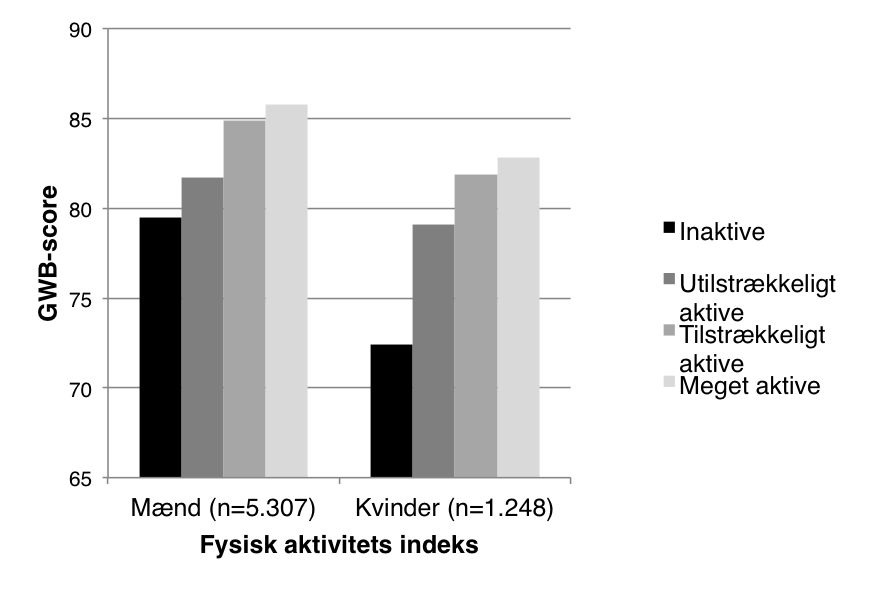
\includegraphics[width=0.6\textwidth]{figures/inaktivitet_gwb}
\caption{Fysisk inaktivitet sammenholdt med følelsesmæssig trivsel. På x-aksen fremgår grupperingen i fysisk aktivitetsniveau for hhv. mænd og kvinder. På y-aksen fremgår den gennemsnitlige GWB-score, hvilket indikerer følelsesmæssig trivsel på en skala fra $0-110$ \citep{galper2006}.}
\label{fig:inaktivitet_gwb}
\end{figure}

\begin{figure}[H]
\centering
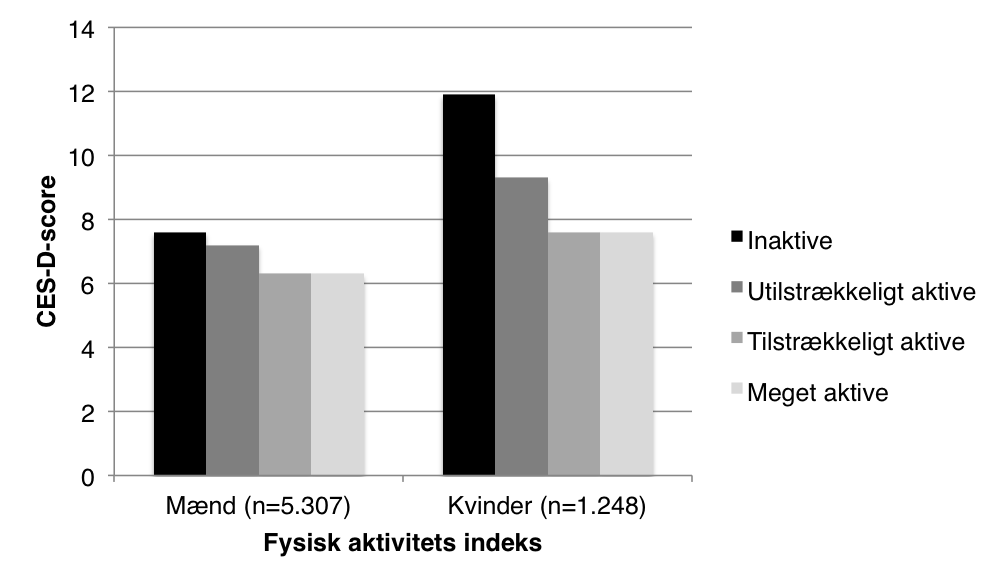
\includegraphics[width=0.6\textwidth]{figures/inaktivitet_dep}
\caption{Fysisk inaktivitet sammenholdt med depressionssymptomer. På x-aksen fremgår grupperingen i fysisk aktivitetsniveau for hhv. mænd og kvinder. På y-aksen fremgår den gennemsnitlige CES-D-score, hvilket indikerer depressive symptomer på en skala fra $0-60$ \citep{galper2006}.}
\label{fig:inaktivitet_dep}
\end{figure}

\noindent
Resultater herfra, som fremgår af \autoref{fig:inaktivitet_gwb} og \autoref{fig:inaktivitet_dep}, viser, at fysisk inaktive, især kvinder, har en højere tendens til depressive symptomer, end andre, der er mere fysisk aktive. På samme måde fremgik det af studiet, at fysisk inaktive forsøgspersoner  ikke trives følelsesmæssigt, som de, der er mere aktive \citep{galper2006}. 

Der er derved en sammenhæng mellem fysisk inaktivitet og psykiske følger, som eksempelvis depression og forværret følelsesmæssig trivsel \citep{galper2006}. Yderligere er der evidens for, at fysisk inaktivitet forværrer allerede eksisterende depressionstilstande samt dårlig følelsesmæssig trivsel \citep{motionsraad2007}.

% Afgrænsning af "sygdommen" til hypertension (en form for indledning til Birgithes afsnit)
\section{Sygdommen}
Det er påvist, at mange sygdomme har gavn af fysisk aktivitet som en behandling eller en metode til at forebygge sygdomsprogression. \citep{motionsraad2007,pedersen2011} Dette gælder forskellige typer sygdomme, og som påvirker forskellige aldersgrupper, hvorfor fysisk aktivitet generelt kan siges at være gavnligt, og hvorfor der eksisterer anbefalinger for alle omkring fysisk aktivitet. \citep{pedersen2011} Af denne grund vælges der til dette projekt at tage udgangspunkt i én sygdom og fysisk aktivitets påvirkning på netop denne sygdom.

Hypertension udgør en risikofaktor for følger som apopleksi, myokardieinfarkt, hjerteinsufcciens samt pludselig død, og ifølge nuværende definitioner af hypertension har omkring 20 \% af befolkningen denne sygdom. \citep{pedersen2011} Fysisk inaktivitet øger risikoen for hypertension, og motion har en synlig blodtrykssænkende effekt. \citep{olsen2015} Af denne grund vælges hypertension som udgangspunktet for dette projekt og denne problemanalyse. 
\section{Hypertension}

Af de 20 \% voksne danskere med hypertension, er omkring 30 \% ikke diagnosticeret. Dette skyldes, at der ofte ikke er tydelige symptomer på lidelsen \cite{kronborg2008}. Symptomer, der kan forekomme ved hypertension, er træthed, hovedpine, næseblod, hjertebanken og åndenød ved anstrengelse. Idet hypertension i de fleste tilfælde ikke medfører symptomer, opdages lidelsen derfor ofte ved et tilfælde \cite{olsen2015}.
% olsen2015: https://www.sundhed.dk/borger/patienthaandbogen/hjerte-og-blodkar/sygdomme/hoejt-blodtryk-hypertension/hypertension-symptomer/ 
% Ikke optimal kilde, men andre kilder siger det sammen, både danske og engelske. 
Der er en række sundhedsmæssige risici forbundet med hypertension, idet sygdommen medfører et øget pres på kroppens blodkar, hvilket forøger risikoen for udvikling af arteriesklerose, aneurismer, hjerteanfald og apopleksi. Længerevarende hypertension er af denne grund ofte årsag til kronisk nyresvigt og hjerte-kar-sygdomme \cite{martini2015}. Det kan være svært at estimere de nøjagtige tal for dødeligheden som følge af hypertension, idet patienterne ofte dør af følgevirkninger heraf, og årsagen til dødsfaldet kan være uklar. Ifølge Statens Institut for Folkesundhed er omkring 4 \% af alle dødsfald i Danmark relateret til hypertension \cite{juel2006}.
 
På trods af de sundhedsmæssige risici ved hypertension får 2/3 af de diagnosticerede patienter ikke tilstrækkelig behandling, således at de kan opnå det anbefalede blodtryk \cite{paulsen2012}.
Blodtryk er karakteriseret ved et systolisk og et diastolisk blodtryk, som henholdsvis er trykket i arterierne, når hjertet trækker sig sammen under systole, og trykket mellem to hjerteslag under diastole. Blodtryk skrives som ”systole/diastole” og måles i enheden millimeter kviksølv (mmHg). Det anbefales, at blodtrykket er under 140/90 mmHg, hvor et blodtryk over denne grænse betegnes hypertension. Er blodtrykket mellem 120/80 og 139/89 mmHg kaldes dette prehypertension, og der bør gøres opmærksom på dette for at undgå hypertension \cite{martini2015}.
% Martinibogen skal i kildelisten.

I de fleste tilfælde er årsagen til hypertension ukendt, men der er patientgrupper, der har særlig høj risiko for at udvikle hypertension. En lidelse, der ofte forbindes med hypertension, er diabetes. De to lidelser er begge resultatet af metabolisk syndrom, som er forstyrrelser i kroppens metabolisme og forekommer ofte grundet overvægt \cite{cheung2012}.

Behandling af hypertension kan ske farmakologisk eller non-farmakologisk. Ved farmakologisk behandling tages der højde for graden af hypertension, samt hvorvidt der er udviklet følgesygdomme. Alle patienter med hypertension bør behandles non-farmakologisk, hvilket betyder de får en række anbefalinger fra lægen, der bør følges. Herunder blandt andet ændring af motions- og kostvaner. Hypertensive patienter bør jævnligt ved konsultationer få kontrolleret blodtrykket, hvor lægen eller sygeplejersken desuden kan følge op på patientens vægt, kost og aktivitetsniveau. Normalt vil hypertension kunne behandles i almen praksis, men i tilfælde af behandlingsresistent hypertension, hvor blandt andet motion, kostændringer og formindsket alkoholindtag ikke kan udrede sygdommen, vil patienterne opleve at blive videresendt til en hypertensionsklinik \cite{lodberg2016, bech2015}.
\section{Nuværende metoder til aktivitetsmåling}

Inden for det danske sygehusvæsen, defineres fysisk aktivitet som værende en aktivitet, der forhøjer energiomsætningen. 
Dette betyder at alt mellem indkøb og gåture, til målrettet fysisk træning, kan defineres som værende fysisk aktivitet.\citep{gupta2013, terkelsen2015}

Sundhedsstyrelsen anbefaler desuden et aktivitetsniveau på mindst 30 minutters motion af moderat intensitet hver dag hele ugen. 
I forbindelse med dette, er moderat densitet blevet defineret som $40-59\%$ af maksimal iltoptagelse, $64-74\%$ af makspuls eller aktivitet, der gør patienten lettere forpustet, uden at forhindre muligheden for samtale. 
For at patienten bliver defineret som værende fysisk inaktiv, kræver det af den grund mindre end $2.5$ timers fysisk aktivitet om ugen.\citep{gupta2013}

I forbindelse med monitorering af aktivitetsniveauet for patienter ved klinikbesøg, kan den fysiske aktivitet bestemmes med udgangspunkt i flere forskellige undersøgelsesmetoder \citep{gupta2013}. 
Måden hvorpå aktiviteten monitoreres, kan opdeles i to kategorier: objektiv og subjektiv \citep{gupta2013, adamo2009}. 

%% Subejtiv metoder - Overordnet

En almindelig subjektiv metode, der anvendes er selvudfyldt dokumentation, der typisk giver et indblik i type af aktivitet, intensitet, hyppighed, samt tidsperiode for ydet aktivitet \citep{adamo2009}. Dertil er der forskellige måder at dokumentere den fysiske aktivitet, som f.eks. en aktivitetslog, aktivitetsdagbog, spørgeskemaer og lignende \citep{adamo2009}. 

%% Subjektive metoder - Konkrete beskrivelser

Spørgeskemaer tager udgangspunkt i faste spørgsmål omhandlende patientens fysiske aktivitet i løbet af dagligdagen \citep{muller2009}. 
Disse omhandler blandt andet transport til og fra arbejde, motionsvaner, tid brugt foran eksempelvis computer eller TV og ønsker om eventuelle ændringer af patientens aktivitetsvaner \citep{gupta2013, vestergaard2012}. 

Alternativt anvendes aktivitetsdagbøger \citep{muller2009} for at opnå en mere fyldestgørende indsigt i patientens aktivitetsmønster \citep{gupta2013}. 
Dagbogen fungerer som en logbog, hvori den primære aktivitet siden sidste notation, nedskrives med bestemte intervaller. 
Denne monitoreringsmetode giver et bedre indblik i patientens fysiske aktivitet gennem dagen, men er også mere tidskrævende at anvende for især patient men også læge.\citep{gupta2013}

%% Subjektive metoder - Overordnet ulemper 

Disse subjektive metode anvendes på grund af dens lave omkostning, lave patientbyrde, og generelle accept, samtidig med at den er velegnet til dokumentation af diversiteten i forhold til hvilken fysisk aktivitet der er ydet \citep{adamo2009}.

Denne type aktivitetsførelse forbindes dog med en fejlrepræsentation i forhold til den reelle fysiske aktivitet. Da det er en subjektiv dokumentationsmetoder, har patienter en tendens til enten at over- eller undervurderer deres egnen fysiske aktivitet \citep{adamo2009}. 
Et studie oplyser at 72 \% af patienter, af alderen 19 eller derunder, overestimerer deres fysiske aktivitet ved selvudfyldelse, i forhold til aktiviteten målt med objektiv/direkte aktivitetsførelse (accelerometer, pedometer, og lignende.) \citep{adamo2009}

Problematikken er således at de subjektive metoder ikke altid er i stand til at repræsentere den reelle fysiske aktivitet, selvom metoderne anses som værende valide \citep{pedersen2011, gupta2013}. 

%%%%%%%%%%%%%%%%%%%%%%%%%%%%%%%%%%%%%%%%%%%%%%%

Som et led i behandling af kronikere, såsom overvægtige eller diabetespatienter, udleveres der også skridttællere (accelerometre)\citep{muller2009, jensen2012, snorgaard2010}. 
Accelerometret vil give et mere detaljeret overblik over patientens aktivitetsmønster end spørgeskemaer og dagbøger, grundet muligheden for at monitorere kontinuert gennem længere tid. 
Der opstår dog komplikationer i forbindelse med anvendelsen, som følge af accelerometrets manglende evne til at opfange forskellige aktiviteter. 
Af den grund anvendes det kun til at danne et billede af, hvor meget tid patienten bruger på generel bevægelse. \citep{gupta2013}
\section{Alternative metoder til aktivitetsmåling}
Udover aktivitetsdagbog kan mere objektive målemetoder såsom pulsmåling, dobbeltmærket vand, accelerometer og skridttæller eller en kombination af flere anvendes til monitorering af aktivitetsniveauet hos individer [1?],\cite{motionsraad2007}. 

Pulsmåler bruges til at måle hjertefrekvensen. Der findes flere forskellige metoder til at detektere pulsen, her i blandt ved at måle den elektriske spændingsforskel som hjertet udsender ved hjælp af elektroder på hudens overflade, denne metode anvender typisk et bælte som brugeren har rundt om thorax \cite{motionsraad2007} [MANGLER]. En anden metode kaldet pulsoximeter, måler iltmætningen i blodet for heraf at kunne registrere pulsen [4?]. 

En pulsmåler indeholder elektroder, og ved kontakt med hudens overflade vil den elektriske spændingsforskel blive målt. 

Selvom pulsmålere giver et godt overblik over pulsfrekvensen ved et moderat eller højere intensitet, indebærer den også en begrænsning, ved registrering af pulsen i forbindelse med inaktivitet ved let aktivitet. For at pulsen ikke bliver påvirket af følelsesmæssige ændringer på kroppen, såsom forskrækkelse, hvor energiforbruget vil afvige lidt,  bruges flex-puls metoden. Denne metode har først en kalibreringsligning som bruges til at bestemme sammenhængen mellem arbejdsintensitet og puls hos den enkelte person. Ud fra kalibreringsligningen findes hvilepulsen, som kan bruges til at finde en flex-puls dvs. gennemsnittet mellem hvilepulsen og pulsen under letteste arbejde. \cite{motionsraad2007}

Dobbeltmærket vand er en metode som måler energiomsætning i kroppen. 

Skridttællerens primær funktion er at vise antal gået skridt indenfor en bestemt afstand. Skridttælleren kan hertil også måle antal forbrændte kalorier, totale træningstid og afstanden som brugeren har gået afhængigt af  designet. Skridttæller kaldes også pedometer, og findes i både mekanisk og elektronisk form. [1?]

Både skridttæller og aktivitetsarmbånd kan patienten monitorere på håndleddet og kan bruges under træning eller i hverdagen. Teknologierne kan bruges i forbindelse med selvkontrol af aktivitetsniveau, hvilket vil betyde at patienten har mere ansvar for monitorering af aktivitetsniveauet. 

Aktivitetsarmbånd, som også er et elektronisk måleinstrument, bruges af forskellige målgrupper for eksempel elite atleter/udøvere, som forbereder eller øver til en konkurrence. Aktivitetsarmbånd kan udover skridttælling også måle fysiske parametre som puls, søvn og kalorieindtag samt kalorier forbrændt. [2?] 

Aktivitetsarmbåndet kan blive synkroniseret til andre enheder såsom computer og mobil, på denne måde kan data også blive overført. 

%Et studie af Eduardo Ferriolli et al (Physical Activity Monitoring: A Responsive and Meaningful Patient-Centered Outcome for Surgery, Chemotherapy, or Radiotherapy?) målte 

%[1] http://www.explainthatstuff.com/how-pedometers-work.html 

%[2] 

%[3]http://sundhedsstyrelsen.dk/publ/MER/2007/FYSISK_INAKTIVITET-KONSEKVENSER_OG_SAMMENHAENGE2007.PDF (objektive målemetoder)

%[4] Pulse Oximetry Training Manual (se under mappen litteratur)

%Alt muligt andet pis:

%“Background: With the ever-increasing availability of health information technology (HIT) enabling health consumers to measure, store, and manage their health data (e.g., self-tracking devices) ”
%FYSISK_INAKTIVITET-KONSEKVENSER_OG_SAMMENHAENGE2007.PDF
\section{Problemformulering}

Her vil være en opsummering af problemanalysen, for at tydeliggøre hvorfor problemformuleringen lyder som følgende:

\textit{Hvilke effekter vil implementeringen af aktivitetsarmbånd til registrering og objektivisering af fysisk aktivitet hos hypertensive patienter have i den almene praksis?}

\textit{Hvilke påvirkninger vil implementeringen af aktivitetsarmbånd i den almene praksis til registrering og objektivisering af fysisk aktivitet have hos hypertensive patienter?}

%-------------MTV--------------------

%-------------Teknoglogi-------------
Teknologi
Dette kapitel har fokus på det teknologiske element, hvor teknologien vil blive karakteriseret, analyseret og vurderet. Dette gøres i henhold til metodeafsnittet (???). Der er opstillet en række MTV spørgsmål, som vil redegøre for og vurdere, om aktivitetsarmbånd fra et teknologisk synspunkt kan anvendes til at måle aktivitetsniveau hos patienter med ’sygdom’. Herudover vil det blive undersøgt, hvilke følgevirkninger anvendelse af aktivitetsarmbånd har på patientens sygdom. (Eller noget??)

Hvordan måles patienters aktivitet på nuværende tidspunkt? (I problemanalysen?)

Hvordan fungerer en aktivitets tracker/armbånd(??), og hvordan kan denne anvendes i medicinsk sammenhæng, således at en almen praktiserende læge får dokumenteret patientens aktivitetsniveau?
(Er der på nuværende tidspunkt læger, der anvender aktivitetsarmbånd, hvordan får de data fra aktivitetsarmbåndet?)

Hvor stor nøjagtighed/pålidelighed er det nødvendigt, at aktivitets armbånd har, hvis de skal anvendes til det ønskede formål, og hvor nøjagtige/pålidelige er de eksisterende aktivitetsarmbånd? (eller omvendt – Hvor nøjagtige er aktivitetsarmbånd, og er pålideligheden stor nok til at kunne anvendes i sundhedssektoren?)

Hvilken effekt (eller konsekvenser, følgevirkninger?) har anvendelsen af aktivitetsarmbånd til dokumentering af aktivitetsniveau på patientens sygdom?

(Hvilke problematikker kan opstå ved brug af aktivitetsarmbånd?) fneh….
% Indhold i afsnittet\\
\section{Besvarelse}
Indhold: Dette afsnit vil indeholde forskellige underemner, der vil beskæftige sig med forskellige aspekter, så MTV-spørgsmålene kan besvares. 
\section{Delkonklusion}
Indhold: Dette afsnit vil indeholde en delkonklusion af denne del af MTV'en og dette kapitel, som forhåbentligt vil lede frem til en endelig konklusion i syntesen. 

%-------------Patient----------------
\chapter{Patienten}
Dette kapitel har fokus på patientaspektet, hvor teknologiens påvirkning på patienten vil blive karakteriseret, analyseret og vurderet. 
\section{Metode}
Til analyse af patienten og hvordan teknologien påvirker denne, anvendes \autoref{fig:patientaspekter}. Her analyseres sociale forhold, kommunikative forhold, økonomiske forhold, individuelle forhold og etiske forhold, samt sammenspillet mellem disse. I forhold til Fitbit Flex lægges der i denne analyse vægt på sociale forhold, herunder hvordan denne teknologi påvirker patientens arbejds- og uddannelsesliv, familie og livskvalitet, individuelle forhold, herunder hvordan patienten oplever teknologien, kommunikative forhold, samt etiske forhold, herunder risiko for misbrug af personlige data. 
%(Nogle af aspekterne kan vægte mere end andre alt efter hvilken teknologi der er tale om, med en aktivitets tracker er det nok mest, (listet i prioriteret rækkefælge) sociale forhold, herunder hvordan det påvirker patientens arbejds/uddannelses liv, familie, fritid og generel livskvalitet. Individuelle forhold, herunder hvordan patienten oplever teknologien, tilfredshed, motivation, tryghed mm. Kommunikative forhold, herunder hvordan der kommunikeres fra f.eks. sygehus til patient og omvendt, fra teknologi til patient og sygehus. Etiske forhold kan måske indgå i og med at patienternes aktivitet måles og bliver opsamlet som data, disse data bliver set af patienten og lægen, måske deler patienten sine resultater over sociale medier, kan disse data misbruges af andre? GPS, placering kan ses. Økonomiske forhold, altså om teknologien giver udgifter for patienten eller påvirker vedkommendes økonomi.).


\begin{figure}[H]
\centering
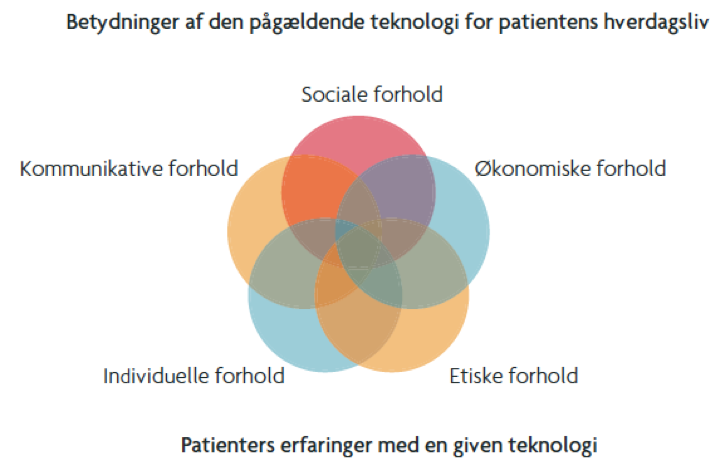
\includegraphics[width=0.8\textwidth]{figures/patientaspekter}
\caption{Patient-aspekter \citep{mtvhaandbog}.}
\label{fig:patientaspekter}
\end{figure}

\noindent
Dette giver anledning til følgende MTV-spørgsmål: 
%(Inklusions og eksklusions kriterier skal muligvis opstilles for at kunne fokusere modellen på den målgruppe som vi vælger at fokusere på)


\subsection{MTV-spørgsmål}
\begin{itemize}
\item Skal der være bestemte kriterier opfyldt for at patienten kan få en aktivitets tracker?
\item Er teknologien brugervenlig og motiverer den patienten til at få en mere aktiv hverdag?
\item Hvordan påvirker teknologien patienternes individuelle og sociale forhold i dagligdagen?
\item Hvor stor en andel af patienter oplever en positiv virkning ved anvendelse af teknologien, hvad er tidshorisonten for denne virkning, og hvad spiller en rolle for at teknologien giver et succesfuldt forløb?
\item Hvor meget ansvar har patienten ved anvendelsen af teknologien?
\item Er der nogle etiske aspekter ved at monitorere patientens aktivitet, i så fald hvilke dilemmaer opstår heraf?
\end{itemize} 


% Indhold i afsnittet
\section{Besvarelse}
Indhold: Dette afsnit vil indeholde forskellige underemner, der vil beskæftige sig med forskellige aspekter, så MTV-spørgsmålene kan besvares. 
\section{Delkonklusion}
Indhold: Dette afsnit vil indeholde en delkonklusion af denne del af MTV'en og dette kapitel, som forhåbentligt vil lede frem til en endelig konklusion i syntesen. 

%-------------Organisation-----------
\chapter{Organisation}
\section{Metode}
En organisationsanalyse har til formål at belyse opbygningen af organisationen, hvori teknologien skal implementeres, i forhold til tilrettelæggelse og opgavefordeling. 
Det ønskes at undersøge de organisatoriske forudsætninger samt mulige (?) konsekvenser ved implementering af et (…)-aktivitetsarmbånd til monitorering i den primære sektor. Dette gøres ud fra et udgangspunkt i den modificerede Leavitt organisationsmodel samt samtaler med alment praktiserende læge (...?) for at analysere konsekvenserne af en eventuel ændring i organisationen. Leavitts modificerede organisationsmodel benyttes, da denne tager højde for omgivelsernes påvirkning på teknologi, aktører, opgaver, struktur, disses indbyrdes påvirkning og påvirkning på omgivelserne.

\begin{figure}[H]
\centering
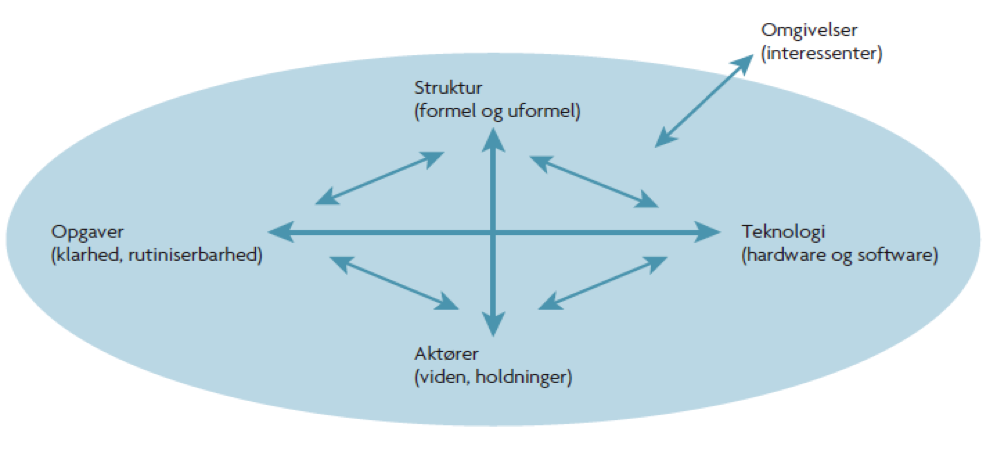
\includegraphics[width=0.9\textwidth]{figures/leavitt}
\caption{Leavitts modificerede organisationsmodel.}
\label{fig:leavittmodel}
\end{figure}

Dette giver anledning til følgende MTV-spørgsmål:

\subsection{MTV-spørgsmål}
\begin{itemize}
\item Hvordan passer  (…)-aktivitetsarmbånd ind i den nuværende organisation? 
\item Hvilke krav vil implementering af (…)-aktivitetsarmbånd stille til alment praktiserende læger, og hvem skal stå for en eventuel efteruddannelse? 
\begin{enumerate}
\item Hvor nemt/svært/tidskrævende er det at analyse data fra et sådant armbånd?
\item Hvornår er det ”nok” aktivitet til, at det kan bruges som et værktøj? Hvor går grænsen, og er det let at se om denne overskrides? 
\item Efteruddannelse/information/oplæg på konference, som kun nogle læger deltager i? Hvad vil dette betyde, hvis man har en ”gammeldags” læge?  Skal det være et tilbud fra alle læger, og hvordan sørger man for dette?
\end{enumerate}
\item  Hvordan vil arbejdsfordelingen mellem den primære og sekundære sundhedssektor blive påvirket, og hvad vil en ændring i arbejdsfordelingen medføre?
\begin{enumerate}
\item Hvor mange patienter bliver på nuværende tidspunkt henvist til sekundære sundhedssektor
\end{enumerate} 
\end{itemize}
% Indhold i afsnittet
\section{Besvarelse}
Indhold: Dette afsnit vil indeholde forskellige underemner, der vil beskæftige sig med forskellige aspekter, så MTV-spørgsmålene kan besvares. 
\section{Delkonklusion}
Indhold: Dette afsnit vil indeholde en delkonklusion af denne del af MTV'en og dette kapitel, som vil lede frem til en endelig konklusion i syntesen. 

%-------------Økonomi----------------
%%%%%%%%%%%%%%%%%%%%%%%%%%%%%%%%%%%%%%%%%%%%%%%%%%%%%%%%
%\chapter{Økonomi}
%Dette afsnit omhandler det økonomiske aspekt ift. MTV analysen.
\chapter{Økonomi}

\section{Metode}
% Hvad koster den patientgruppe for samfundet? Hvad koster det, hvis de ikke passer deres sygdom ordentlig (i forhold til motion), og dermed får følgevirkninger (fx hospitalsophold, medicin)? (Cost/Benefit analyse??)
% Cost-effectiveness analysen (konsekvenserne måles i naturlige enheder)
%Cost-utility analysen (konsekvenserne måles i kvalitetsjusterede leveår (QALYs))
% Cost-benefit analysen (konsekvenserne opgøres i kroner og øre)
% Hvordan er omkostningerne sammenlignet med alternativerne?
% I forlængelse af, hvad aktivitetstrackeren skal kunne: Er de billige tilstrækkelige, eller er det nødvendigt at købe de dyre?
% Brugerbetaling eller egenbetaling??

I økonomianalysen undersøges hvilke omkostninger der er forbundet med anvendelse af aktivitetsmåler som dokumenteringsenhed for aktivitet i den almene praksis/medicin.
Ligeledes undersøges omkostninger for nuværende anvendelsesmetoder, samt hvilke økonomiske konsekvenser der forekommer når patienten ikke opretholder anbefalet aktivitetskvote.
Dette er med henblik på at fremhæve sundhedsgevinsterne i forhold til udgifterne.   
Omkostningerne og konsekvenser er opgjort af sundhedsøkonomiske analyser, som cost-effectiveness analyse (CEA), cost-utility analyse (CUA) og cost-benefit analyse (CBA), og oplyses i henholdsvis narturlige enheder (f.eks. vunde leveår), kvalitetsjusterede leveår og kroner øre. 
De estimerede værdier fra de forskellige analyser er baseret på eksisterende litteratur samt basale økonomiske udregninger.
Dette giver anledning til følgende MTV-spørgsmål: 

\subsection{MTV-spørgsmål}
%Eksempler
%\begin{itemize}
%\item Hvad vil forskellige modeller for vaccinationsprogram have af nytteeffekten i forhold til omkostninger?

%\item Hvordan ville en eventuel screening påvirke organisering og økonomi? 

%\item Hvad er de ressourcemæssige konsekvenser?
%\end{itemize}

\noindent  
\begin{itemize}
\item Hvad er omkostningerne ved nuværende anvendelsesmetoder, samt konsekvenserne ved utilstrækkelig aktivitetsydelse? 

\item Hvilke omkostninger er forbundet med brug af aktivitetsarmbånd til (?)-patienter, og hvad er den økonomiske konsekvens af dette, hvis brug af aktivitetsarmbånd resulterer i et øget antal kvalitetsjusterede leveår?

%\item Hvilke samfundsøkonomiske ændringer er der forbundet ved udlevering af aktivitetsmålere til patienter med ???.

%\item Hvordan ville et aktivitetsarmbånd påvirke organisering og økonomi?

%\item Hvilke omkostninger er forbundet med kvantificering af patientaktivitet, i forhold til nuværende anvendelsesmetoder (Aktivitetslog)?.  


\end{itemize}
 




% Indhold i afsnittet
\section{Besvarelse}
Indhold: Dette afsnit vil indeholde forskellige underemner, der vil beskæftige sig med forskellige aspekter, så MTV-spørgsmålene kan besvares. 
\section{Delkonklusion}
Indhold: Dette afsnit vil indeholde en delkonklusion af denne del af MTV'en og dette kapitel, som forhåbentligt vil lede frem til en endelig konklusion i syntesen. 

%-------------Syntese--------------------
\chapter{Syntese}
\section{Diskussion}
\chapter{Konklusion}

Som konklusion på MTV'en besvares projektets problemformulering:

~
\begin{center}
\textit{Hvilke påvirkninger vil implementeringen af Fitbit Flex i den almene praksis til registrering og objektivisering af fysisk aktivitet have hos hypertensive patienter i sundhedssektoren?}
\end{center}
~

\noindent I MTV-analysen er det fundet, at brugen af Fitbit Flex i den primære sektor, vil give de praktiserende læger et mere objektivt grundlag for vurdering af hypertensive patienters aktivitetsniveau. Sammenlignet med den nuværende metode, hvor der primært anvendes spørgeskemaer, vil implementeringen af Fitbit Flex resultere i, at eventuel bias ved vurderingen af aktivitetsmønstret forsvinder som følge af, at patienternes aktivitet kvantificeres.

På baggrund af de undersøgte studier kan det påvises, at anvendelsen af aktivitetsarmbånd har potentialet til at resultere i en mere aktiv hverdag, som følge af den motiverende faktor i forbindelse med en forøget indsigt i eget aktivitetsmønster. Ud fra dette kan det konkluderes, at implementeringen af Fitbit Flex kan have en positiv indvirkning på hypertensive patienters aktivitetsniveau, hvilket kan forbedre patienternes tilstand, men dette kræver yderligere undersøgelser.

Ved implementering af Fitbit Flex vil patientforløbet og antallet af videresendelser fra primær til sekundær sektor kunne påvirkes. Dette sker som følge af, at patienterne har mulighed for at opnå en sundere livsstil ved anvendelse af armbåndet, hvorfor færre vil opleve en forværring af den hypertensive tilstand. Derved er det en mulighed at holde dem i den primære sektor, hvor der anvendes livsstilsændringer og blodtryksmedicin uden indlæggelser til behandling af sygdommen. Implementeringen vil påvirke den primære sektor i form af efteruddannelse til de indblandede parter, der skal udlevere armbåndet og instruere patienter i anvendelsen af teknologien.

Trods den motiverende faktor, som giver mulighed for et forhøjet aktivitetsniveau, vil Fitbit Flex ikke være et alternativ til anden behandling. Aktivitetsarmbåndet vil i stedet fungere som et hjælpemiddel til både læger og patienter, hvor det giver bedre vurderingsgrundlag og potentiale til sundere livsstil, som vil kunne betyde, at færre patienter videresendes ved forværring af hypertension.
\chapter{Anbefalinger}
Indhold: Dette afsnit kan indeholde nogle anbefalinger, hvis rapportens konklusion ender med at lede frem til nogle.

%-------------Bibliografi--------------------

\begingroup \label{litteratur}
\raggedright
\bibliographystyle{unsrtnat}
\bibliography{bibliography/bibliography}
\endgroup


%-------------Bilag-------------------------
\begin{appendices}
\chapter{Søgeprotokol}\label{app:soegeprotokol}
Indhold: Dette appendiks vil indeholde søgeprotokol for rapportens forskellige afsnit. Dette sættes ind, når søgningerne er udført. 
\end{appendices}



\end{document}